\documentclass[14pt]{beamer}
\usepackage{etex}
%%%%%%%%%%%%%%%%%%%%%%%%%%%%%%%%%%%%%%%%%%%%%%%%%%%%%%%%%%%%%
\usepackage[ngerman]{babel}
\usepackage[T1]{fontenc}
\usepackage[utf8]{inputenc}
%%%%%%%%%%%%%%%%%%%%%%%%%%%%%%%%%%%%%%%%%%%%%%%%%%%%%%%%%%%%%
% Meta informations:
\newcommand{\trauthor}{Louis Kobras}
\newcommand{\trtype}{Proseminar} %{Proseminar} %{Seminar} %{Workshop}
\newcommand{\trcourse}{Knowledge Processing with Neural Networks}
\newcommand{\trtitle}{Generieren dynamischer Antworten durch Parsing von natürlicher Sprache}
\newcommand{\trmatrikelnummer}{6658699}
\newcommand{\tremail}{4kobras@informatik.uni-hamburg.de}
\newcommand{\trinstitute}{Dept. Informatik -- Knowledge Technology, WTM}
\newcommand{\trwebsiteordate}{{http://www.informatik.uni-hamburg.de/WTM/}}
%%%%%%%%%%%%%%%%%%%%%%%%%%%%%%%%%%%%%%%%%%%%%%%%%%%%%%%%%%%%%
% Bind packages:
\usepackage{beamerthemesplit}
\usetheme{Boadilla}
%\usetheme{Copenhagen}
%\usetheme{Darmstadt}
%\usetheme{Frankfurt}
%\usetheme{Ilmenau}
%\usetheme{JuanLesPins}
%\usetheme{Madrid}
%\usetheme{Warsaw }
%\usecolortheme{dolphin}
%\setbeamertemplate{sections/subsections in toc}[sections numbered]
%\beamertemplatenavigationsymbolsempty
%\setbeamertemplate{headline}[default] 	% deaktiviert die Kopfzeile
\setbeamertemplate{navigation symbols}{}% deaktiviert Navigationssymbole
%\useinnertheme{rounded}

\usepackage{tikz}
\usepackage{pgf}
\usetikzlibrary{arrows,automata,positioning}

\usepackage{acronym}                    % Acronyms
\usepackage{algorithmic}				% Algorithms and Pseudocode
\usepackage{algorithm}					% Algorithms and Pseudocode
\usepackage{amsfonts}                   % AMS Math Packet (Fonts)
\usepackage{amsmath}                    % AMS Math Packet
\usepackage{amssymb}                    % Additional mathematical symbols
\usepackage{amsthm}
\usepackage{color}                      % Enables defining of colors via \definecolor
\usepackage{fancybox}                   % Gleichungen einrahmen
\usepackage{fancyhdr}										% Paket zur schickeren der Gestaltung der 
\usepackage{graphicx}                   % Inclusion of graphics
%\usepackage{latexsym}                  % Special symbols
\usepackage{longtable}					% Allow tables over several parges
\usepackage{listings}                   % Nicer source code listings
\usepackage{caption}
\usepackage{lmodern}
\usepackage{multicol}					% Content of a table over several columns
\usepackage{multirow}					% Content of a table over several rows
\usepackage{rotating}					% Alows to rotate text and objects
\usepackage[section]{placeins}          % Ermoeglich \Floatbarrier fuer Gleitobj. 
\usepackage[hang]{subfigure}            % Allows to use multiple (partial) figures in a fig
%\usepackage[font=footnotesize,labelfont=rm]{subfig}	% Pictures in a floating environment
\usepackage{tabularx}										% Tables with fixed width but variable rows
\usepackage{url,xspace,boxedminipage}   % Accurate display of URLs
\usepackage{ulem}
\usepackage{soul}

\definecolor{uhhRed}{RGB}{254,0,0}		  % Official Uni Hamburg Red
\definecolor{uhhGrey}{RGB}{136,136,136} % Official Uni Hamburg Grey
\definecolor{uhhLightGrey}{RGB}{180,180,180} % Official Uni Hamburg LightGrey
\definecolor{uhhLightLightGrey}{RGB}{220,220,220} % Official Uni Hamburg LightLightGrey
\definecolor{pblue}{rgb}{0.13,0.13,1}
\definecolor{pgreen}{rgb}{0,0.5,0}

\setbeamertemplate{itemize items}[ball]
\setbeamercolor{title}{fg=uhhRed,bg=white}
\setbeamercolor{title in head/foot}{bg=uhhRed}
\setbeamercolor{block title}{bg=uhhGrey,fg=white}
\setbeamercolor{block body}{bg=uhhLightLightGrey,fg=black}
\setbeamercolor{section in head/foot}{bg=black}
\setbeamercolor{frametitle}{bg=white,fg=uhhRed}
\setbeamercolor{author in head/foot}{bg=black,fg=white}
\setbeamercolor{author in footline}{bg=white,fg=black}
\setbeamercolor*{item}{fg=uhhRed}
\setbeamercolor*{section in toc}{fg=black}
\setbeamercolor*{separation line}{bg=black}
\setbeamerfont*{author in footline}{size=\scriptsize,series=\mdseries}
\setbeamerfont*{institute}{size=\footnotesize}


\lstset{ %
language=Java,   							% choose the language of the code
basicstyle=\small\ttfamily,  				% the size of the fonts that are used for the code
numbers=left,                   			% where to put the line-numbers
numbersep=5pt,                  			% how far the line-numbers are from the code
backgroundcolor=\color{light-light-gray},   % choose the background color. You must add
frame=lrtb,           						% adds a frame around the code
tabsize=4,          						% sets default tabsize to 2 spaces
captionpos=b,           					% sets the caption-position to bottom
breaklines=true,        					% sets automatic line breaking
xleftmargin=1.5cm,							% space from the left paper edge
commentstyle=\color{pgreen},
keywordstyle=\color{pblue},
literate=%
    {Ö}{{\"O}}1
    {Ä}{{\"A}}1
    {Ü}{{\"U}}1
    {ß}{{\ss}}1
    {ü}{{\"u}}1
    {ä}{{\"a}}1
    {ö}{{\"o}}1
    {~}{{\textasciitilde}}1
}
\renewcommand{\lstlistingname}{Code}
\captionsetup[lstlisting]{font={footnotesize},margin=1.5cm,singlelinecheck=false } % removes "Listing 1: "
\definecolor{light-light-gray}{gray}{0.95}


\newcommand{\opticalseperator}{0.0025\paperwidth}

\institute{Universit\"at Hamburg\\\trinstitute}
\title{\trtitle}
\subtitle{\trtype}
\author{\trauthor}
\date{}
\logo{}

%%%%%%%%%%%%%%%%%%%%%%%%%%%%%%%%%%%%%%%%%%%%%%%%%%%%%%%%%%%%%
% Configurationen:
%\hypersetup{pdfpagemode=FullScreen}

\hyphenation{whe-ther} 									% Manually use: "\-" in a word: Staats\-ver\-trag

%\lstloadlanguages{C}                   % Set the default language for listings
\DeclareGraphicsExtensions{.pdf,.svg,.jpg,.png,.eps} % first try pdf, then eps, png and jpg
\graphicspath{{./src/}} 								% Path to a folder where all pictures are located

%%%%%%%%%%%%%%%%%%%%%%%%%%%%
% Costom Definitions:
\setbeamertemplate{title page}
{
  \vbox{}
	\vspace{0.4cm}
  \begin{centering}
    \begin{beamercolorbox}[sep=8pt,center,colsep=-4bp]{title}
      \usebeamerfont{title}\inserttitle\par%
      \ifx\insertsubtitle\@empty%
      \else%
        \vskip0.20em%
        {\usebeamerfont{subtitle}\usebeamercolor[fg]{subtitle}\insertsubtitle\par}%
      \fi%     
    \end{beamercolorbox}%
		\vskip0.4em
    \begin{beamercolorbox}[sep=8pt,center,colsep=-4bp,rounded=true,shadow=true]{author}
      \usebeamerfont{author}\insertauthor \\ \insertinstitute
    \end{beamercolorbox}

	  \vfill
	  \begin{beamercolorbox}[ht=8ex,center]{}
		  
\includegraphics[width=0.20\paperwidth]{wtmIcon.pdf}
	  \end{beamercolorbox}%
    \begin{beamercolorbox}[sep=8pt,center,colsep=-4bp,rounded=true,shadow=true]{institute}
      \usebeamerfont{institute}\trwebsiteordate
    \end{beamercolorbox}
		\vspace{-0.1cm}
  \end{centering}
}

\setbeamertemplate{frametitle}
{
\begin{beamercolorbox}[wd=\paperwidth,ht=3.8ex,dp=1.2ex,leftskip=0pt,rightskip=4.0ex]{frametitle}%
		\usebeamerfont*{frametitle}\centerline{\insertframetitle}
	\end{beamercolorbox}
	\vspace{0.0cm}
}

\setbeamertemplate{footline}
{
  \leavevmode
	\vspace{-0.05cm}
  \hbox{
	  \begin{beamercolorbox}[wd=.32\paperwidth,ht=4.8ex,dp=2.7ex,center]{author in footline}
	    \hspace*{2ex}\usebeamerfont*{author in footline}\trauthor
	  \end{beamercolorbox}%
	  \begin{beamercolorbox}[wd=.60\paperwidth,ht=4.8ex,dp=2.7ex,center]{author in footline}
	    \usebeamerfont*{author in footline}\trtitle
	  \end{beamercolorbox}%
	  \begin{beamercolorbox}[wd=.07\paperwidth,ht=4.8ex,dp=2.7ex,center]{author in footline}
	    \usebeamerfont*{author in footline}\insertframenumber{}
	  \end{beamercolorbox}
  }
	\vspace{0.15cm}
}

%%%%%%%%%%%%%%%%%%%%%%%%%%%%
% Additional 'theorem' and 'definition' blocks:
\newtheorem{axiom}{Axiom}[section] 	
%\newtheorem{axiom}{Fakt}[section]			% Wenn in Deutsch geschrieben wird.
%Usage:%\begin{axiom}[optional description]%Main part%\end{fakt}

%Additional types of axioms:
\newtheorem{observation}[axiom]{Observation}

%Additional types of definitions:
\theoremstyle{remark}
%\newtheorem{remark}[section]{Bemerkung} % Wenn in Deutsch geschrieben wird.
\newtheorem{remark}[section]{Remark} 

%%%%%%%%%%%%%%%%%%%%%%%%%%%%
% Provides TODOs within the margin:
\newcommand{\TODO}[1]{\marginpar{\emph{\small{{\bf TODO: } #1}}}}

%%%%%%%%%%%%%%%%%%%%%%%%%%%%
% Abbreviations and mathematical symbols
\newcommand{\modd}{\text{ mod }}
\newcommand{\RS}{\mathbb{R}}
\newcommand{\NS}{\mathbb{N}}
\newcommand{\ZS}{\mathbb{Z}}
\newcommand{\dnormal}{\mathit{N}}
\newcommand{\duniform}{\mathit{U}}

\newcommand{\erdos}{Erd\H{o}s}
\newcommand{\renyi}{-R\'{e}nyi}

%%%%%%%%%%%%%%%%%%%%%%%%%%%%
% Display of TOCs:
\AtBeginSection[]
{
	\setcounter{tocdepth}{2}  
	\frame
	{
	  \frametitle{Outline}
		\tableofcontents[currentsection]
	}
}
 
%%%%%%%%%%%%%%%%%%%%%%%%%%%%%%%%%%%%%%%%%%%%%%%%%%%%%%%%%%%%%
% Document:
\begin{document}
\renewcommand{\arraystretch}{1.2}

\begin{frame}[plain] % plain => kein Rahmen
  \titlepage
\end{frame}
%\setcounter{framenumber}{0}

\frame{
	\frametitle{Outline}
	\tableofcontents
}


%%%%%%%%%%%%%%%%%%%%%%%%%%%%%%%%%%%%%%%%%%%%%%%%%%%%%%%%%%%%%
%%%%%%%%%%%%%%%%%%%%%%%%%%%%%%%%%%%%%%%%%%%%%%%%%%%%%%%%%%%%%
%%%%%%%%%%%%%%%%%%%%%%%%%%%%%%%%%%%%%%%%%%%%%%%%%%%%%%%%%%%%%
%%%%%%%%%%%%%%%%%%%%%%%%%%%%%%%%%%%%%%%%%%%%%%%%%%%%%%%%%%%%%
%%%%%%%%%%%%%%%%%%%%%%%%%%%%%%%%%%%%%%%%%%%%%%%%%%%%%%%%%%%%%
%%%%%%%%%%%%%%%%%%%%%%%%%%%%%%%%%%%%%%%%%%%%%%%%%%%%%%%%%%%%%

%%%%%%%%%%%%%%
% Your Content

\section{Motivation und Frage}

\frame[t]{
	\frametitle{Motivation}
	\begin{itemize}
		\item Schaffen eines Systems zum Verständnis natürlicher Sprache
		\item Einbindung ebenjenes Systems in Videospiele für mehr Interaktion
		\item Bezug auf Text-Adventures
	\end{itemize}
}

\section{Grundlagen und Definition}
\frame[t]{
	\frametitle{Natürliche Sprache I}
	\textit{''By 'natural language' we mean a language that is used for everyday communication by humans;
				languages such as English, Hindi, or Portuguese.
        In contrast to artificial languages such as programming languages and mathematical notations,
        	natural languages have evolved as they pass from generation to generation,
        	and are hard to pin down with explicit rules.''} (Bird, 2009)
}
\frame[t]{
	\frametitle{Natürliche Sprache I}
	\textit{''By 'natural language' we mean a language that is \textcolor{pgreen}{used for everyday communication} by humans;
				languages such as English, Hindi, or Portuguese.
        In contrast to artificial languages such as programming languages and mathematical notations,
        	natural languages \textcolor{pgreen}{have evolved} as they pass from generation to generation,
        	and are \textcolor{pgreen}{hard to pin down with explicit rules}.''} (Bird, 2009)
}
\frame[t]{
	\frametitle{Natürliche Sprache II}
	\begin{itemize}
		\item Morphologie
		\item Syntax
		\item Semantik
		\item Pragmatik
		\item Diskurs
		\item Mehrdeutigkeit
		\item Phonologie
	\end{itemize}
	(Liste nach Jurafski, Martin, 2009; Definitionen nach Duden)
}
\frame[t]{
	\frametitle{Natürliche Sprache II}
	\begin{itemize}
		\item \textbf{\underline{Morphologie}}
		\item Syntax
		\item Semantik
		\item Pragmatik
		\item Diskurs
		\item Mehrdeutigkeit
		\item \st{Phonologie}
	\end{itemize}
	(Liste nach Jurafski, Martin, 2009; Definitionen nach Duden)
}
\frame[t]{
	\frametitle{Status Quo}
	\begin{center}
	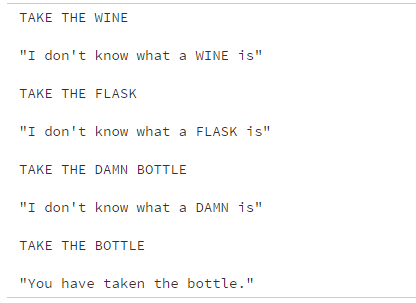
\includegraphics[scale=0.7]{dialogue.png}
	\end{center}
	\footnotesize
	(\textit{NPC Conversations})
}

\section{Ansatz}
\frame[t]{
	\frametitle{Gewählte Vorgehensweise}
	\begin{itemize}
		\item Analyse des ELIZA-Programms
		\item Analyse natürlicher Sprache
		\item Suchen von Hilfsmitteln zum Analysieren von Sprache
		\item Umwandeln einer Eingabe in verwertbare Daten
		\item Mithilfe von ELIZA auf die Daten reagieren
	\end{itemize}
}
\frame[t]{
	\frametitle{ELIZA}
	Was ist ELIZA?\\
	\begin{itemize}
		\item Chatbot
		\item simuliert einen Psychologen
		\item entstanden 1966 am MIT
		\item Grundlage der dynamischen Text-/Sprachverarbeitung
		\item erste Schritte in angewandter KI
	\end{itemize}
}
\frame[t]{
	\frametitle{ELIZA}
	Arbeitsweise von ELIZA\\
	\begin{itemize}
		\item Text-Input erhalten
		\item Input nach Schlüsselwörtern absuchen
		\item Input nach Regeln analysieren
		\item mithilfe von Regeln aus Schlüsselwörtern Antworten generieren
	\end{itemize}
}
\frame[t]{
	\frametitle{DFAs}
	\begin{figure}[h]
	\label{fig:dfa}
		\begin{tikzpicture}[->,>=stealth',shorten >=1pt,auto,node distance=3.0cm,semithick]
			\node	[initial, state]	(q0)								{$q_0$};
			\node	[state]				(q1)	[right of=q0]				{$q_1$};
			\node	[accepting, state]	(q2)	[right of=q1]				{$q_2$};
			\node	[accepting, state]	(q3)	[below of=q0,yshift=0.5cm]	{$q_3$};
			\node	[state]				(q4)	[right of=q3,xshift=4cm]	{$ERR$};

			\path
				(q0)	edge					node	[align=center]	{1. Buchstabe \\ groß}			(q1)
				(q1)	edge					node	[align=center]	{Stamm in \\ Nomen}				(q2)
				(q2)	edge	[in=90,out=220]	node	[align=center]	{endet \\ auf \textbf{n}}		(q3)
				(q2)	edge	[loop right]	node	[align=center]	{Gültiges \\ Affix}				(q2)
				(q3)	edge					node	[align=center]	{~~~~Wort nicht \\ ~~~~zu Ende}	(q4)
				(q1)	edge					node	[align=center]	{}								(q4)
			;
		\end{tikzpicture}
		\footnotesize
		\caption{DFA zur Zerlegung des Wortes \textit{Nachkommastellen} in seine Morpheme}
	\end{figure}
}
\frame[t]{
	\frametitle{DFAs}
	\begingroup
	\centering
	\begin{figure}[h]
	\label{tab:morphemes}
	\begin{tabular}{ccccc}
		N	&	(n)ach	&	komma	&	stelle	&	n	\\
		N	&	+pref	&	+stamm	&	+suff	&	+PL	
	\end{tabular}\\
	\-\\
	\textit{Nachkommastellen} und die dazugehörige Morphemkette
	\end{figure}
	\endgroup
}
\frame[t]{
	\frametitle{RegEx}
	\begin{itemize}
		\item	\string[A-Z].*
		\item	\string[a-z].*
		\item	.*n
		\item	.*\textbackslash\textbackslash d+.+
		\item	.+\textbackslash\textbackslash d+.*
		\item	.+\textbackslash\textbackslash d+.+
		\item	.
		\item	\textbackslash\textbackslash d\textbackslash\textbackslash d*?
	\end{itemize}
}
\frame[t]{
	\frametitle{Java String}
	\begin{itemize}
		\item contains
		\item indexOf
		\item substring
		\item length
	\end{itemize}
}

\section{Ergebnis}
\frame[t]{
	\frametitle{Folgende Vorgehensweise}
	\begin{itemize}
		\item Mithilfe der genannten Hilfsmittel die Wörter der Eingabe auf ihre Grundformen zurückführen
		\item Diese Grundformen mit der Schlüsselwortliste von ELIZA abgleichen
		\item Die zusätzlich gewonnen Informationen nutzen, um den Kontext zu interpretieren
		\item Einen Kontext für eine Antwort schaffen
		\item Die Regeln von ELIZA anwenden, um eine Antwort zu generieren
	\end{itemize}
}

\section{Schlussfolgerung}

\frame[t]
{
	\frametitle{Abschluss I}
	Es wurde gezeigt:
	\begin{itemize}
		\item Funktionsweise von ELIZA
		\item Erweiterbarkeit von ELIZA mithilfe von programmiererischen Hilfsmitteln
		\item Funktion und Benutzung dieser Hilfsmittel
		\item Anwendbarkeit im gewählten Gebiet, namentlich der Spieleentwicklung
  	\end{itemize}
\mbox{ }
}

\frame[t]{
	\frametitle{Abschluss II}
	Weiteres Vorgehen:\\
	\begin{itemize}
		\item Analysieren der anderen genannten Aspekte
		\item Kombinieren der Aspekte zu einem natürliche Sprachen verstehenden System
	\end{itemize}
}

%%%%%%%%%%%%%%
\frame[c]{
	\frametitle{Literatur}
	\footnotesize
	Literatur:
	\begin{itemize}
		\item Daniel Jurafski, James H. Martin, \textit{Speech and Language Processing}, Prentice Hall, 2009
		\item Hauke Stieler, \textit{Windows 10: Warum Microsoft sich verzählt hat}, Blogpost, Juni 2015
		\item Joseph Weizenbaum, \textit{ELIZA - A Computer Program for thr Study of Natural Language Communication between Man and Machine}, in \textit{Communications of the ACM, 9(1):36-45}, Januar 1966
		\item Dudenredaktion, \textit{Duden - Die deutsche Rechtschreibung}, Dudenredaktion, Oktober 2014
		\item Steven Bird, Ewan Klein, Edward Loper, \textit{Natural language Processing with Python}, O'Reilly Media, Inc, 2009
		\item Unknown Author, edited by Amit Patel, \textit{NPC Conversations}, Stanford University, Dept. of Computer Science
	\end{itemize}
}

%%%%%%%%%%%%%%

\frame[c]{
  \frametitle{The End}
\begin{center}
  Danke für eure Aufmerksamkeit.\\[1ex]
  Fragen?\\[5ex]
\end{center}
	\-\\
	\-\\
	\footnotesize
	Präsentation und Paper abrufbar auf\\
	\textcolor{pblue}{\url{https://github.com/4kobras/Homework/blob/master/Pros_KI/}}
}


%%%%%%%%%%%%%%%%%%%%%
%####	ANHANG	####%
%%%%%%%%%%%%%%%%%%%%%

\frame[plain]{
	\frametitle{ELIZA}
	\footnotesize
	\[
		(a)\text{ It seems that}~~~~(b)\text{ you}~~~~(c)\text{ hate}~~~~(d)\text{ me}
	\]
	\-\\
	\[
		(f)\text{What makes you think that}~~~~(d)\text{ I}~~~~(c)\text{ hate}~~~~(b)\text{ you}
	\]
	\-\\
	\[
		(0)~~~~\text{YOU}~~~~(0)~~~~\text{ME}~~~~\longrightarrow~~~~(0)~~~~\text{I}~~~~(3)~~~~\text{YOU}
	\]
	\pause
	\-\\
	\-\\
	\[
		(0)~~~~\text{YOU}~~~~(0)~~~~\longrightarrow~~~~(0)~~~~\text{I}~~~~(3)
	\]
}
\frame[plain]{
	\frametitle{ELIZA}
	\centering
	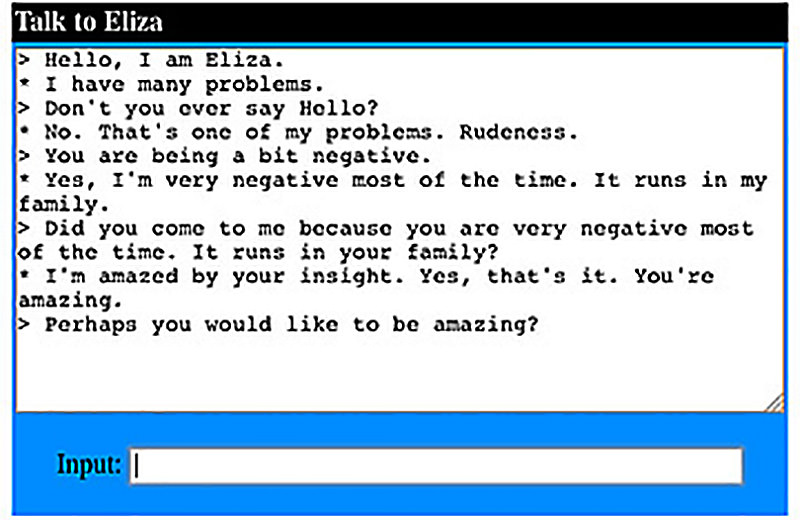
\includegraphics[scale=0.35]{Eliza-dialogue-5.jpg}\\
	\footnotesize
	Quelle: https://www.olark.com/img/uploads/Eliza-dialogue-5.jpg
}



\end{document}
